\documentclass[11pt]{beamer}
\usetheme{Pittsburgh}
\usepackage[utf8]{inputenc}
\usepackage[spanish]{babel}
\usepackage{amsmath}
\usepackage{amsfonts}
\usepackage{amssymb}
\usepackage{graphicx}
\author{Luis Greco - Marcela Herrera - Cristian Kubrak - Alejo Salvador }
\title{Trabajo Práctico 3}
\subtitle{Tomografía computada}
%\setbeamercovered{transparent} 
%\setbeamertemplate{navigation symbols}{} 
%\logo{} 
%\institute{} 
%\date{} 
%\subject{} 
\begin{document}



\begin{frame}
\titlepage 
\end{frame}


\begin{frame}{INTRODUCCIÓN}
\begin{itemize}
\item El objetivo de este trabajo práctico es evaluar un método para reconstruir imágenes tomográficas sujetas a ruido, utilizando el método de aproximación por cuadrados mínimos.
\end{itemize}
\end{frame}

\begin{frame}{PREMISAS}
\begin{itemize}
\item Nuestro sujeto es una imagen de $n$x$n$ pixeles discretizada en celdas de $d$x$d$ pixeles.
\item La intensidad de un pixel se asocia al tiempo que demora un rayo en atravesar ese pixel.
\item La distancia que recorre un rayo que atraviesa al sujeto es igual a la cantidad de pixeles por los que pasa.
\item En cinemática $Velocidad = Espacio/Tiempo$. En este caso la ''velocidad'' promedio dentro de la celda $k$ es:
\begin{displaymath}
v_{k} =(\sum_{i=1}^{n}\sum_{j=1}^{n} I_{[i][j]})/n*n
\end{displaymath}
\item Los rayos están sujetos a ruido.
\end{itemize}
\end{frame}


\begin{frame}{DESARROLLO}
\frametitle {Discretización}
\begin{itemize}
\item Utilizamos valores divisores de la dimensión de la limagen (100 x 100 pixeles).
\item En los tests de granularidad, variamos el tamaño de las celdas tomando los valores 4x4, 5x5, 10x10, 20x20, 25x25 y 50x50 pixeles.
\item A medida que se achica el tamaño de las celdas crece el tiempo de procesamiento, lo cual condicionó la elección de los parámetros.
\end{itemize}
\end{frame}


\begin{frame}
\frametitle{Recorrido de un rayo}
\begin{itemize}
\item Los rayos son considerados como rectas en el plano, caracterizados por un punto de origen que llamamos $(x_{0},y_{0})$ y un ángulo $\alpha$.
\item Se busca la intersección con la recta $y=0$ la cual es el punto $(x-y/tangent(\alpha),0)$.
\item Usando la ecuación de la recta $y=tan(\alpha)*x+y_{0}$ y variando el valor de $x$, se calculan los puntos del plano por los que pasa el rayo.
\item Si el punto hallado pertenece a la imagen se guardan las coordenadas del pixel correspondiente en un vector
\item Se usa el vector para el cálculo de distancias y de tiempos.
% agregar grafico
\end{itemize}
\end{frame}

\begin{frame}
\frametitle{Recorrido de un rayo}
% TODO INCLUIR GRAFICO (VER SI SE PUEDE REUSAR EL SCRIPT DE MATLAB DE LOS % RAYOS ALEATORIOS)
\end{frame}



\begin{frame}
\frametitle{Distancia recorrida por un rayo por celda}
\begin{itemize}
\item A partir del vector de pixeles por los que pasa un rayo, se averigua a qué celda pertenece. Se suma 1 unidad por pixel. El resultado se almacena en la matriz de distancias (una fila por rayos, una columna por celda numeradas de arriba hacia abajo y de izquierda a derecha).
\item Cada rayo toca a lo sumo $2n-1$ celdas. Se usa la estructura de matriz esparza del TP1.
\end{itemize}
\end{frame}


\begin{frame}
\frametitle{Distancia recorrida por un rayo por celda}
% TODO INCLUIR GRAFICO
\end{frame}


\begin{frame}
\frametitle{Velocidad de un rayo}
\begin{itemize}
\item A partir del vector de pixeles por los que pasa un rayo, se acumulan las intensidades de los mismos. Se almacenan los resultados en un vector de ''tiempos''. (un elemento por rayo).
\end{itemize}
\end{frame}

\begin{frame}
\frametitle{Sistema de ecuaciones}
% TODO INCLUIR MATRIZ DE ECUACIONES REALES Y DE CUADRADOS MINIMOS
% COMENTAR RELACION ENTER GRANULARIDAD, TAMAÑO DE LA MATRIZ Y CON EL TIEMPO DE PROCESAMIENTO
\end{frame}


\begin{frame}
\frametitle{Generación de rayos}
\framesubtitle{Cantidad y ubicación de los emisores}
% COMENTAR LAS ELECCIONES FALLIDAS. 
% SI SE PUEDE GRAFICARLAS
% DESCRIBIR SELECCION DE UBICACIONES Y CANTIDAD DE EMISORES Y DE RAYOS
% MENCIONAR LOS VALORES UTILIZADOS EN LA EXPERIMENTACION
\end{frame}


\begin{frame}
\frametitle{Generación de rayos}
\framesubtitle{Cantidad y ubicación de los emisores}
\begin{figure}[H] 
\centering
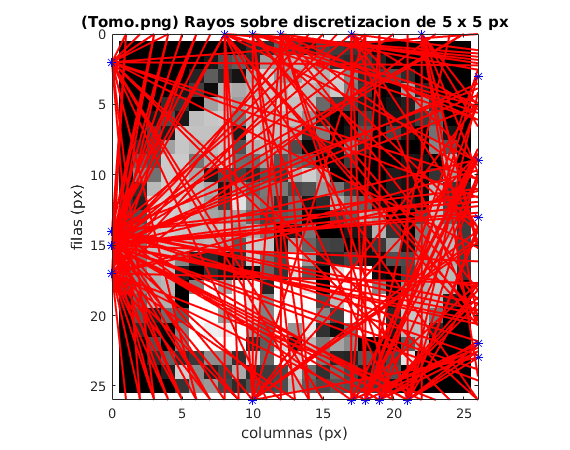
\includegraphics[scale=0.5]{img/rayos_tomo25x25px.png}
\caption{Trazado aleatorio de rayos}
\label{fig:rayos aleatorios}
\end{figure}
\end{frame}


\begin{frame}
\frametitle{Ruido}
% DESCRIBIR COMO SE ELIGIO  PONERLO EN EL VECTOR INDEP
% DESCRIBIR ELECCION DEL CALCULO DEL RUIDO
% MENCIONAR VALORES UTILIZADOS EN LA EXPERIMENTACION
\end{frame}


\begin{frame}{RESULTADOS}
\frametitle{ECM vs. tamaño de la celda}
% incluir graficos e imagenes reconstruidas
\end{frame}



\begin{frame}
\frametitle{ECM vs. cantidad de emisores}
\end{frame}

\begin{frame}
\frametitle{ECM vs. cantidad de rayos por emisor}
\end{frame}


\begin{frame}
\frametitle{Tiempo vs. ???}
\end{frame}


\begin{frame}
\frametitle{Comparacion de resultados}
% comparatica de imagenes con rayos de las esquinas y de la forma que %usanmos finalmente
\end{frame}

\begin{frame}{CONCLUSIONES}
\end{frame}

\begin{frame}{FIN}
\end{frame}



%\begin{frame}
%\tableofcontents
%\end{frame}


\end{document}

